\documentclass[sigconf,review]{acmart}
\usepackage{amssymb}
\usepackage{pifont} % for \cmark and \xmark
\usepackage{pifont} % for \cmark and \xmark
\newcommand{\cmark}{\ding{51}} % check mark
\newcommand{\xmark}{\ding{55}} % cross mark

\usepackage{amsmath,amssymb,amsfonts,latexsym}
\usepackage{enumerate}
\usepackage{lipsum}
\usepackage{xspace}
\usepackage{epsf,picinpar}
\usepackage{hyperref}
\usepackage{varioref}
\usepackage{varioref}
\usepackage{tabularx}
\usepackage{colortbl,multirow,hhline}
\usepackage{listings}
\usepackage{amssymb}
\usepackage{colortbl,multirow,hhline}
\usepackage{algorithmic}
\usepackage{algorithm}
\usepackage{caption}
\usepackage[normalem]{ulem}
\usepackage{cleveref}
\usepackage{xcolor}
\usepackage{pifont}
\usepackage{xcolor,colortbl}
\usepackage{url}
\usepackage{balance}
\usepackage{graphicx, subfigure}
\usepackage{longtable}
\usepackage{lscape}
\usepackage{multirow}
\usepackage{listings}
\usepackage{framed}
\usepackage{morefloats}
\usepackage[T1]{fontenc}
\usepackage{array}
\usepackage{pdfpages}
\usepackage{fancybox}
\usepackage{amsmath}
\usepackage{flushend}
\usepackage{booktabs}
\usepackage{enumitem}

\renewcommand{\ttdefault}{cmr}

%\newcommand{\limit}[1]{\textcolor{red}{\noindent \ding{46}~Page limit:~#1}\\}
\newcommand{\todo}[1]{\textcolor{blue}{\ding{46}~#1}} 
\newcommand{\ie}{\emph{i.e.,}\xspace}
\newcommand{\eg}{\emph{e.g.,}\xspace}
\newcommand{\etc}{etc.\xspace}
\newcommand{\etal}{\emph{et~al.}\xspace} 

\copyrightyear{2025}
\acmYear{2025}
% \setcopyright{acmcopyright}
\acmConference[Green Lab 2025/2026]{Green Lab 2025/2026 - Vrije Universiteit Amsterdam}{September--October, 2025}{Amsterdam, The Netherlands}
\acmBooktitle{Green Lab 2025/2026 - Vrije Universiteit Amsterdam, September--October, 2025, Amsterdam (The Netherlands)}
    
\begin{document}

\begin{figure*}
    \centering
    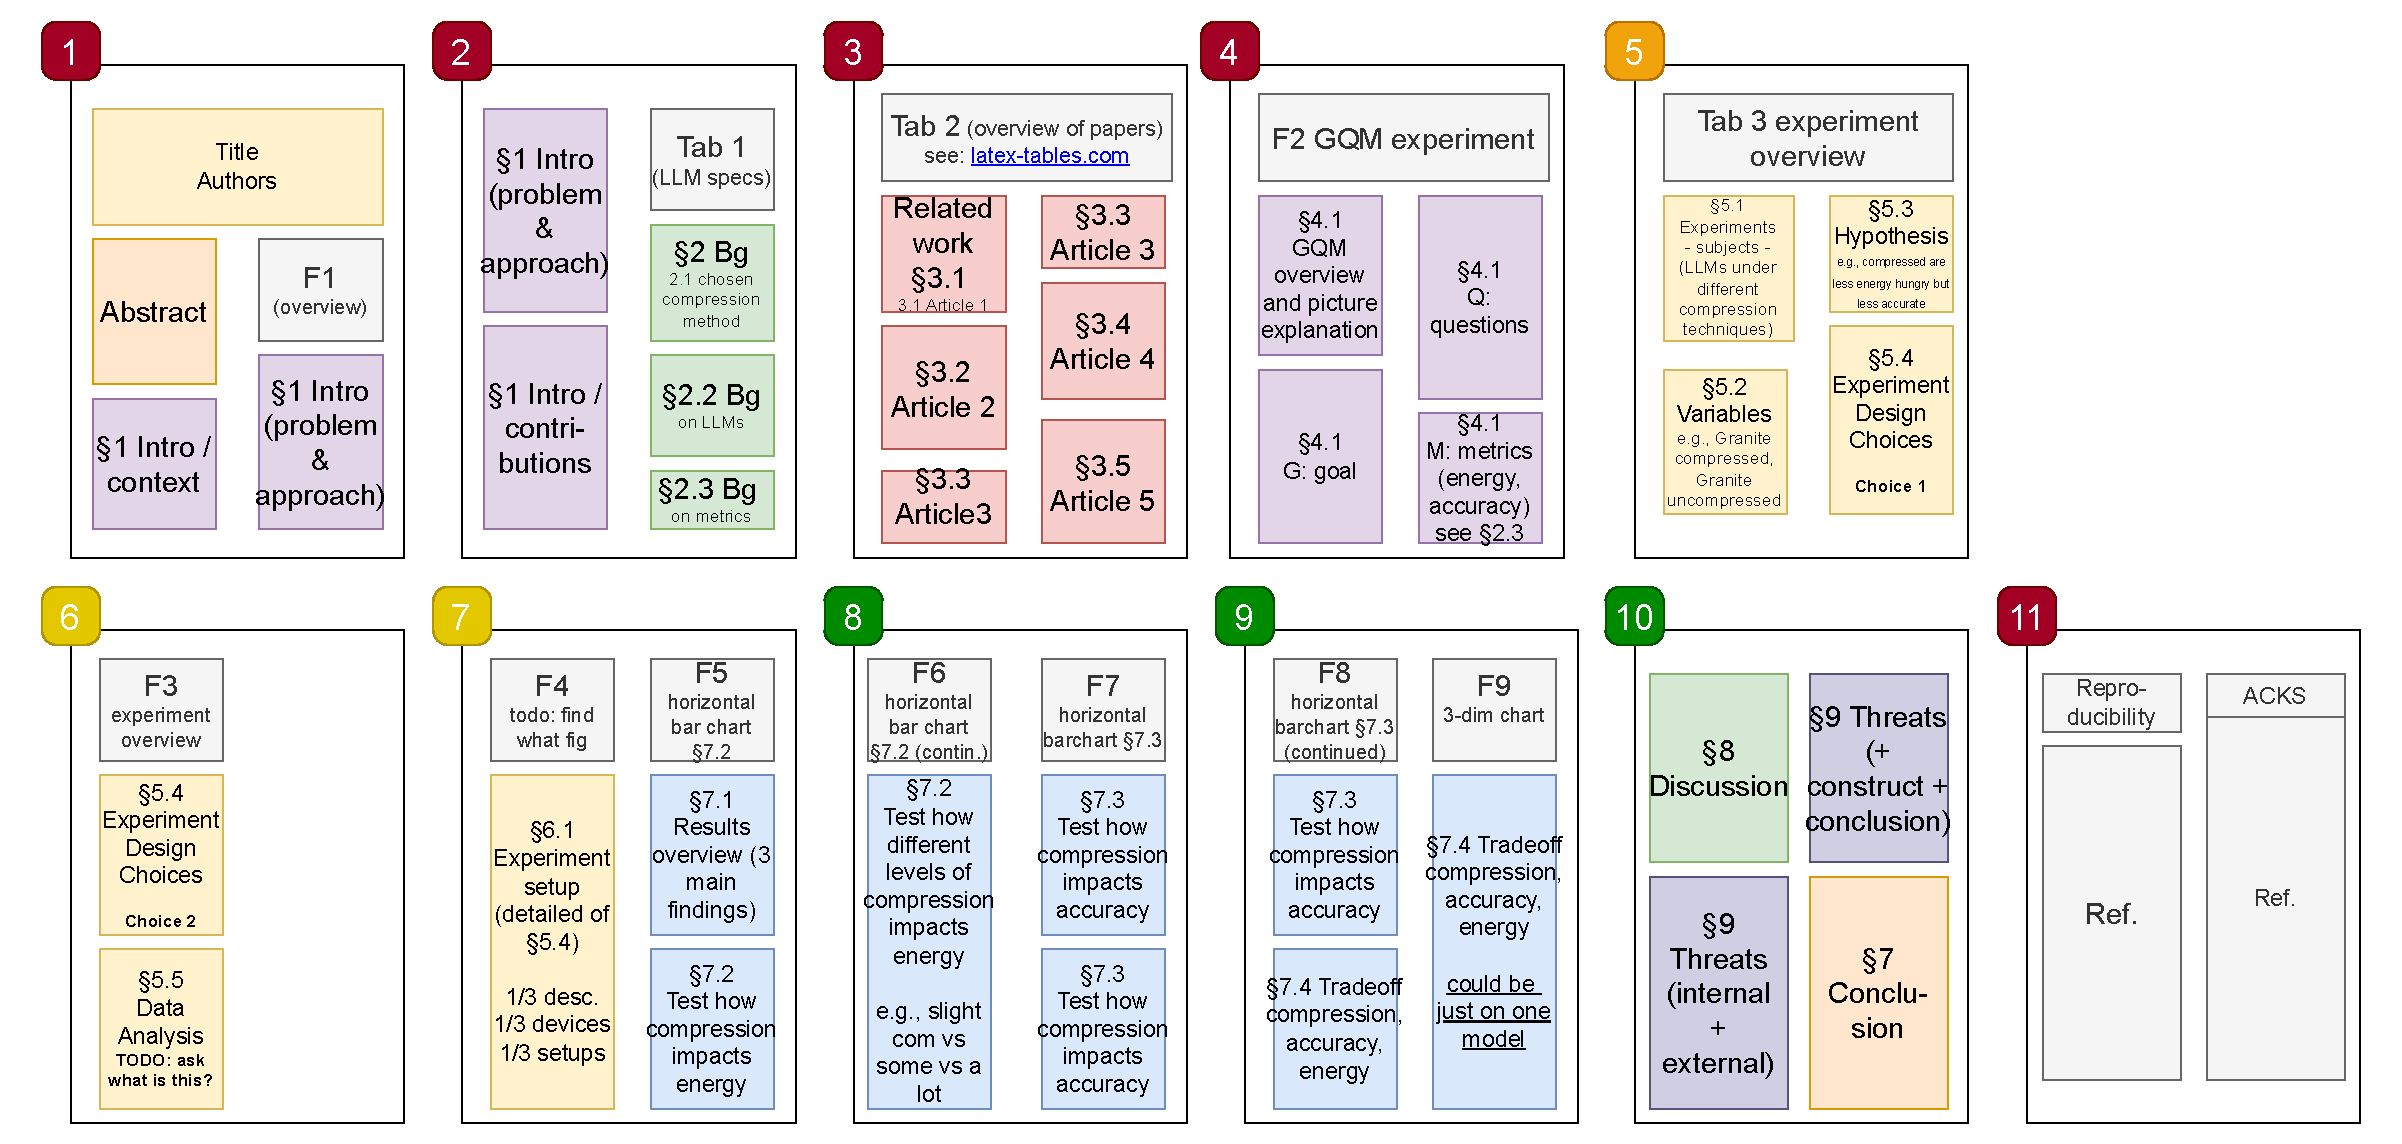
\includegraphics[width=0.95\linewidth]{reportTemplate/figures/paper-page-budgeting-green-lab.pdf}
    \caption{Paper Page Budgeting following the template suggested in the work in progress paper by Iosup et al. in \cite{iosup-epema-systems-writing-wip}. Edit link: \url{https://drive.google.com/file/d/1-9jcqbOQJRCJZpWZldTrm27HNUFuAtWR/view?usp=drive_link}.}
    \label{fig:placeholder}
\end{figure*}

\newpage

\title{
Exploring the impact of LLM compression by quantization on energy consumption, resource utilisation, and accuracy
}

\author{Radu Nicolae}
\affiliation{%
 \institution{2760443 \\ VU Amsterdam, \\ Universiteit van Amsterdam}
} \email{r.nicolae@vu.nl}

\author{Junaid Khalil}
\affiliation{%
 \institution{2891638 \\ VU Amsterdam, \\
 Universiteit van Amsterdam}
} \email{j.khalil6@student.vu.nl}

\author{Muhammad Shayan}
\affiliation{%
 \institution{2891482 \\ VU Amsterdam}
} \email{m.shayan@student.vu.nl}

\author{Md Tasluf Morshed}
\affiliation{%
 \institution{2890836 \\ VU Amsterdam}
} \email{m.t.morshed@student.vu.nl}

\author{Alp Eren Inceoglu}
\affiliation{%
 \institution{2842116 \\ VU Amsterdam}
} \email{a.e.inceoglu@student.vu.nl}

\begin{abstract}
% \noindent \textit{Context}. 
% \todo{at the end}


Large Language Models (LLMs) are being increasingly adopted by our digital society, but raise sustainability concerns when operated at a massive societal scale. % societal context
To improve the performance, efficiency, and, thus, sustainability of LLMs, compression techniques have been widely adopted, yet at the cost of accuracy. % LLM context
One such technique is quantisation, a state-of-the-art approach to reduce model size (thus computation requirements), while maintaining sufficient accuracy, and without architectural changes or re-training. % quantization context
However, although quantization is theoretically expected to generate tradeoffs between energy efficiency, resource utilization (e.g., CPU, memory, inference time), and accuracy degradation, these tradeoffs are insufficiently understood and unquantified. % gap 1
The quantification challenge is further exacerbated by the absence of benchmarking systems for systematically quantifying LLM ecosystems; the lack of such systems can be costly and could misguide operators of LLM services. % gap 2
Addressing the open challenge, in this work, we propose \underline{Quanti}, the first tool for \underline{quanti}fying the sustainability and performance of LLMs. % approach (following AtLarge, community-standard methodology on designing distributed (eco)systems)
We propose an architecture for deploying, measuring, and comparing LLM on the server side. % design
Through experiments with a prototype, % implement
we % evaluate & experiment
(i) explore the impact of quantization on operational-level metrics of LLMs,
(ii) evaluate the tradeoff between energy consumption-accuracy of LLMs underlying different architectures, both original and under compression by quantization, and
(iii) quantify the impact of carbon-aware workload scheduling of compressed and uncompressed models. 
Quanti, together with all the production data, results, and reproducibility capsule, are released open-source on \url{https://github.com/Radu-Nicolae/Quanti}.



% \noindent \textit{Goal}. 
% \todo{at the end}

% \noindent \textit{Method}. 
% \todo{at the end}

% \noindent \textit{Results}. 
% \todo{at the end}

% \noindent \textit{Conclusions}. 
% \todo{at the end}
\end{abstract}

\maketitle

\section{Introduction}

\textbf{MRQ:} How to explore the impact of compression by quantization of LLMs and how this technique impacts energy consumption, resource utilization, and accuracy?

\textbf{RQ1:} How to design and implement a benchmarking system for quantifying LLMs?

\textbf{RQ2:} How to evaluate the impact of compression by quantization of operational-level metrics of LLMs?

\textbf{RQ3:} How to evaluate the tradeoff accuracy-energy consumption across various-architecture LLMs under quantization and without qunatization?

\textbf{RQ4:} How to evaluate the impact of carbon intensity compressed and uncompressed models at favourable and unfavourable carbon intensity day instances?

Carbon intesity 
- night is the worst
- day is the best



This document represents a template of the final experiment report structure for the course \textit{Green Lab} at the Vrije Universiteit Amsterdam \cite{greenlab}.

The experiment is conducted according to the guidelines by Wohlin and colleagues \cite{wohlin12, DBLP:books/sp/WohlinRHORW24}.

The total length of this document must not exceed 15 pages, including references, appendixes, \etc

In this section you have to describe 
(i) the domain (\eg mobile apps and their market) and the technologies relevant for understanding the rest of the document, 


(ii) the main motivation behind your experiment (the problem, here you can show examples via apps/tools screenshots, snippets of source code, \etc), 

(iii) what your experiment is about (hint of the solution), and 

(iv) what the developers will learn from the results of your experiment.  

\textcolor{red}{Page limit: 2}
 \newpage
\section{Background: quantization and quantification} \label{sec:background}

\begin{figure}
    \centering
    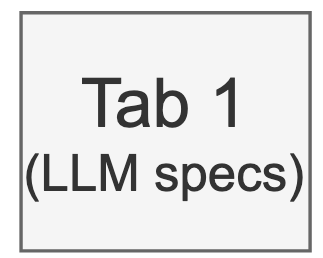
\includegraphics[width=0.75\linewidth]{reportTemplate/figures/f2.png}
    \caption{Caption}
    \label{fig:background}
\end{figure}

In this section, we present background on LLM quantisation and a high-level overview of this compression technique in~\Cref{fig:background}. Then, we present background on metrics and techniques used to quantify accuracy, energy consumption, and CO2 emissions. 

Quantization is \textit{"the division of a quantity into a discrete number of small parts, often assumed to be integral multiples of a common quantify``}~\cite{DBLP:journals/corr/abs-2411-0253}. In LLMs, quantization is a compression technique that reduces the precision of model parameters from standard representation (e.g., 32-bit floating point) to lower-bit representation (e.g., 8-bit integers). Post-training quantization (PTQ) is preferred, primarily due to
the extensive computational demands associated with fine-tuning for Quantization Aware Training~\cite{zhang2023dual, DBLP:conf/icml/NagelABLB20, DBLP:journals/corr/abs-2006-10518}. In this work, we adopt PTQ as our compression method, thus adhering to the state-of-the-art in the community.

We use metrics for quantifying operational-level metrics. We adhere to international system measurements and community standards and quantify energy consumption in kilowatt-hour (kWh) and CO2 emissions in grams of CO2. To derive CO2 emission from energy consumption, we follow the vetted approach proposed by Niewenhuis et al. in Footprinter~\cite{DBLP:conf/wosp/NiewenhuisTIM24}; we present this formula in \Cref{eq:CO2-emissions}, where $C_e$ is the total amount of CO2 emissions, $C_i$ is the carbon intensity, and $E$ is the total energy consumption.

\vspace*{-0.7cm}
\begin{align}
    C_{e} = C_{i} \times E
    \label{eq:CO2-emissions}
\end{align}
\vspace*{-0.6cm}

To quantify accuracy, we will be using Evaluate  library for python, which is a tool to apply many different and well-accepted accuracy metrics, such as BLEU, which is often used to evaluate machine-translations or F1 score, which is the harmonic mean of precision and recall. Since different metrics are best suited to different uses of the LLM, we decided that using ‘Evaluate’s metric collection interface would be the most efficient option. 
	
For the metrics, while this is subject to change, we have decided to use BLEU, F1 and BERT-score, and evaluating these various results to not only find which LLM’s are the most accurate, but also in which categories they are most affected by the compression.




\section{Related Work}\label{sec:related}

\begin{table*}[ht]
    \centering
    \begin{tabular}{lllllll}
        \hline
        \textbf{Study} & \textbf {Quantization} & \textbf{Other technique} & \textbf{Energy Metrics} & \textbf{Accuracy} & \textbf{Resource Usage} & \textbf{CO2 Intensity}\\
        \hline
        \midrule
        Zhu et al. \cite{DBLP:journals/tacl/ZhuLLMW24} & \cmark & \cmark & \xmark & \xmark & \xmark & \xmark\\
        Afrin et al.\cite{DBLP:journals/corr/abs-2507-09665} & \cmark (AWQ) & \xmark & \xmark & \cmark (qual.) & \xmark & \xmark\\
        Khan et al.\cite{DBLP:journals/corr/abs-2504-06307} & \cmark & \xmark & \cmark & \cmark & \xmark & \xmark\\
        Agrawal et al.\cite{10968787} & \cmark & \cmark & \xmark & \cmark & \cmark & \xmark\\
        Yuan et al.\cite{DBLP:conf/cain/YuanSZCZSM24} & \xmark & \cmark (KD) & \cmark & \cmark & \cmark & \xmark\\
        \textbf{Our Work} & \cmark (PTQ) & \xmark & \cmark & \cmark & \cmark & \cmark\\
        \hline
        \bottomrule
    \end{tabular}
    \caption{Gap Analysis of Related Work on LLM Compression}
    \label{tab:gapanalysis}
\end{table*}

This section discusses scientific papers such as our experiment and their contributions, and how our study differs from or extends theirs. We present in \Cref{tab:gapanalysis} an overview and high-level comparison between the metrics of focus accross the analyzed papers.

Zhu et al. \cite{DBLP:journals/tacl/ZhuLLMW24} present a comprehensive review of LLM compression methods like quantization, pruning, knowledge distillation, and low-rank factorization. They elaborate on methods like Quantization-Aware Training (QAT) and Post-Training Quantization (PTQ) and propose benchmarking on FLOPs, inference time, and compression ratio. While their study aggregates existing methods, the present research presents an explicit empirical investigation of quantization, evaluating its overall effects on energy, resources, and accuracy.

Saima Afrin et al. \cite{DBLP:journals/corr/abs-2507-09665} conducted an empirical study examining the impact of Activation-aware Weight Quantization (AWQ) on the qualitative properties of automatically generated code by Large Code Models (LCMs), a custom sub-family of LLMs. In their work, employing cutting-edge static analysis tools, they observed that quantization has a tendency to preserve functional correctness of generated code and qualitative attributes like maintainability, readability, and structural complexity. They further examined the influence of model size on quality degradation following quantization, disproving the belief that loss of information from quantization damages such features. Afrin et al.'s study is especially focused on code quality as applied to Large Code Models, evaluating accuracy primarily in functional correctness and qualitative code properties. Our experiment broadens the perspective, checking the quantization's effect on a broader set of LLM uses (not just code creation) and quantitatively correlating it with measurably consumed energy and several resource consumption metrics, along with functional and qualitative correctness.

Khan et al. \cite{DBLP:journals/corr/abs-2504-06307} evaluate local inference and quantization for reducing the CO2 footprint of LLMs by as much as 45 percent less energy usage and minimal losses in accuracy. They concentrate on sustainability metrics, while we broaden the scope to also include memory, speed, and qualitative performance metrics.

Agrawal et al. \cite{10968787} investigate pruning, quantization, and distillation to deploy LLMs at the edge. They show quantization to be capable of reducing memory usage in half and lowering inference latency. In comparison to their multi-pronged strategy, our technique separates quantization to uncover its specific role in making efficiency-accuracy trade-offs.

Ye Yuan et al. \cite{DBLP:conf/cain/YuanSZCZSM24} estimated empirically the impact of \textbf{Knowledge Distillation} on the energy usage and efficiency of NLP models, such as BERT and GPT-2. They found that their distilled models consumed less energy, took less time to make inferences, and, in some cases, consumed less CPU and memory compared to non-distilled models. The work emphasized the importance of model selection to energy efficiency and performance, particularly for mobile and resource-limited applications. The central theme of Yuan et al.'s paper \cite{DBLP:conf/cain/YuanSZCZSM24} is knowledge distillation as the compression method. Our own experiment, however, specifically targets quantization compression of LLMs. we want to quantify its individual effects on energy consumption, different types of resource consumption measurement, and prediction performance, thus targeting a different but complementary compression setting.

Briefly speaking, prior work establishes the strengths of compression and optimization to efficiency and sustainability. Nevertheless, most survey many approaches, emphasize domain-specific tasks, or focus on other directions. Our work fills this gap by providing an end-to-end, empirical study of quantization's impact on LLMs on energy consumption, resource use, and accuracy
\section{Experiment Definition}
Report about the GQM (with figure).

\textcolor{red}{Page limit: 2}



\section{Experiment Planning}

\subsection{Subjects Selection}
\subsection{Experimental Variables}
\subsection{Experimental Hypotheses}
\subsection{Experiment Design}
\subsection{Data Analysis}

\textcolor{red}{Page limit: 3}
 s
\section{Design of Quanti}\label{sec:design}

\subsection{Requirement Analysis}

\subsection{Design choices}

\textcolor{red}{Page limit: 1}
 s
\section{Experiment Execution}
Report about: how you plan to conduct your experiment, which tools you are going to use, which devices/laptops, figure and description of the overall software/hardware infrastructure you are setting up for the experiment (\eg who communicates with whom, proxies, network requests, order of actions, \etc). 


\subsection{Ealuating quantization impact on operational-level metrics}\label{sec:experiments:operational-level} \label{sec:exp1}

\subsection{Evaluating accuracy-energy tradeoff for various-architectural LLMs, with and without compression}\label{sec:experiments:accuracy-energy} \label{sec:exp2}

\subsection{Evaluating CO2-aware scheduling against compression techniques}\label{sec:experiments:co2-aware} \label{sec:exp3}


\textcolor{red}{Page limit: 2}


\section{Results}
Provide:
\begin{itemize}
\item descriptive statistics
\item hypothesis testing
\end{itemize}
Provide suitable plots and tables to illustrate your results.

\textcolor{red}{Page limit: Open - go deep as you wish}
\section{Discussion}
Report implications and interpretations of your results (possibly grouped by research question).

\textcolor{red}{Page limit: 1}

\section{Threats To Validity}\label{sec:threats}
Report about each type of threat to the validity of the experiment, according to the classification discussed in class.

\subsection{Internal Validity}
\subsection{External Validity}
\subsection{Construct Validity}
\subsection{Conclusion Validity}

\textcolor{red}{Page limit: 1}


\section{Conclusions}\label{sec:conclusions}

One brief paragraph for summarizing the main findings of the report.

One brief paragraph about the possible extensions of the performed experiment (imagine that other 3 teams will be assigned to the extension of your experiment).    

\bibliographystyle{IEEEtran}
\bibliography{references}

\end{document}
